\documentclass[11pt, oneside]{article}   	% use "amsart" instead of "article" for AMSLaTeX format
\usepackage{geometry}                		% See geometry.pdf to learn the layout options. There are lots.
\geometry{letterpaper}                   		% ... or a4paper or a5paper or ... 
%\geometry{landscape}                		% Activate for for rotated page geometry
%\usepackage[parfill]{parskip}    		% Activate to begin paragraphs with an empty line rather than an indent
\usepackage{graphicx}				% Use pdf, png, jpg, or eps� with pdflatex; use eps in DVI mode
								% TeX will automatically convert eps --> pdf in pdflatex		
\usepackage{amssymb}
\usepackage{amsmath}
\usepackage{parskip}
\usepackage{color}

\title{Vector products}
%\author{The Author}
%\section{}
% \subsection*{R code}
\date{}							% Activate to display a given date or no date

\graphicspath{{/Users/telliott_admin/Dropbox/Tex/png/}}

% \begin{center} 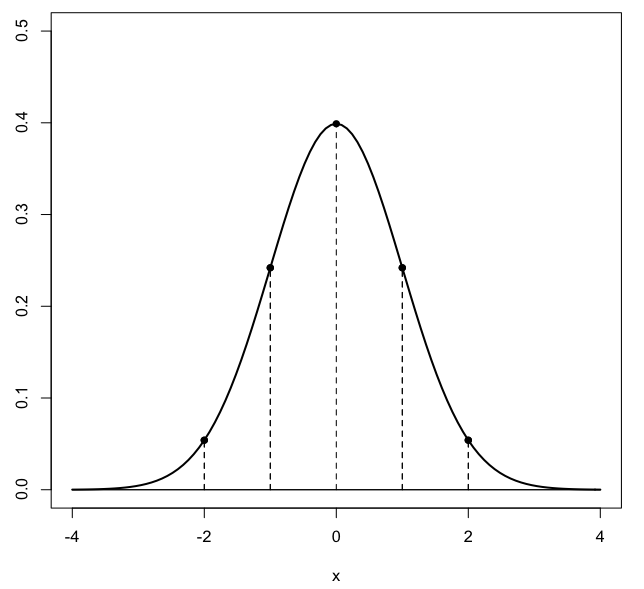
\includegraphics [scale=0.4] {gauss3.png} \end{center}

\begin{document}
\maketitle
\Large
\noindent

In this short write-up I want to explore the algebraic manipulation of vectors, including a brief review of the dot product (sometimes called the \emph{inner} product), and a more detailed look at the cross (vector) product.

Define two vectors $\mathbf{a}$ and $\mathbf{b}$:
\[ \mathbf{a} = \ \langle a_1, a_2 \dots \ a_n \rangle \]
\[ \mathbf{b} = \ \langle b_1, b_2 \dots \ b_n \rangle \]

The dot product is the sum of the products of the individual terms
\[ \mathbf{a} \cdot \mathbf{b} = a_1 b_1 + a_2 b_2 + \dots \ a_n b_n \]
\[ = \sum_i a_i b_i \]
The dot product of two vectors is a number, in vector terminology it is called a \emph{scalar}.  The result may be positive, or negative or even zero.

The dot product of a vector with itself is the square of the length or magnitude
\[ \mathbf{a} \cdot \mathbf{a} = a_1 a_1 + a_2 a_2 + \dots \ a_n a_n \]
(this is just the extension of the Pythagorean theorem to three or more dimensions).  

There is another definition of the dot product which can be shown to be equivalent:
\[ \mathbf{a} \cdot \mathbf{b} = |\mathbf{a}| |\mathbf{b}| \cos \theta \]
The dot product is equal to the magnitude of $\mathbf{a}$ times the magnitude of $\mathbf{b}$ times the cosine of the angle between them.  (Note that this definition indicates that the dot product must be independent of the coordinate system).

A proof of this statement about the dot product comes from the law of cosines.  

For a triangle with sides $a$, $b$ and $c$ and angles opposite those sides $A$, $B$ and $C$, divide the third side into two lengths $c=d+e$ using the vertical altitude from vertex $C$.
\begin{center} 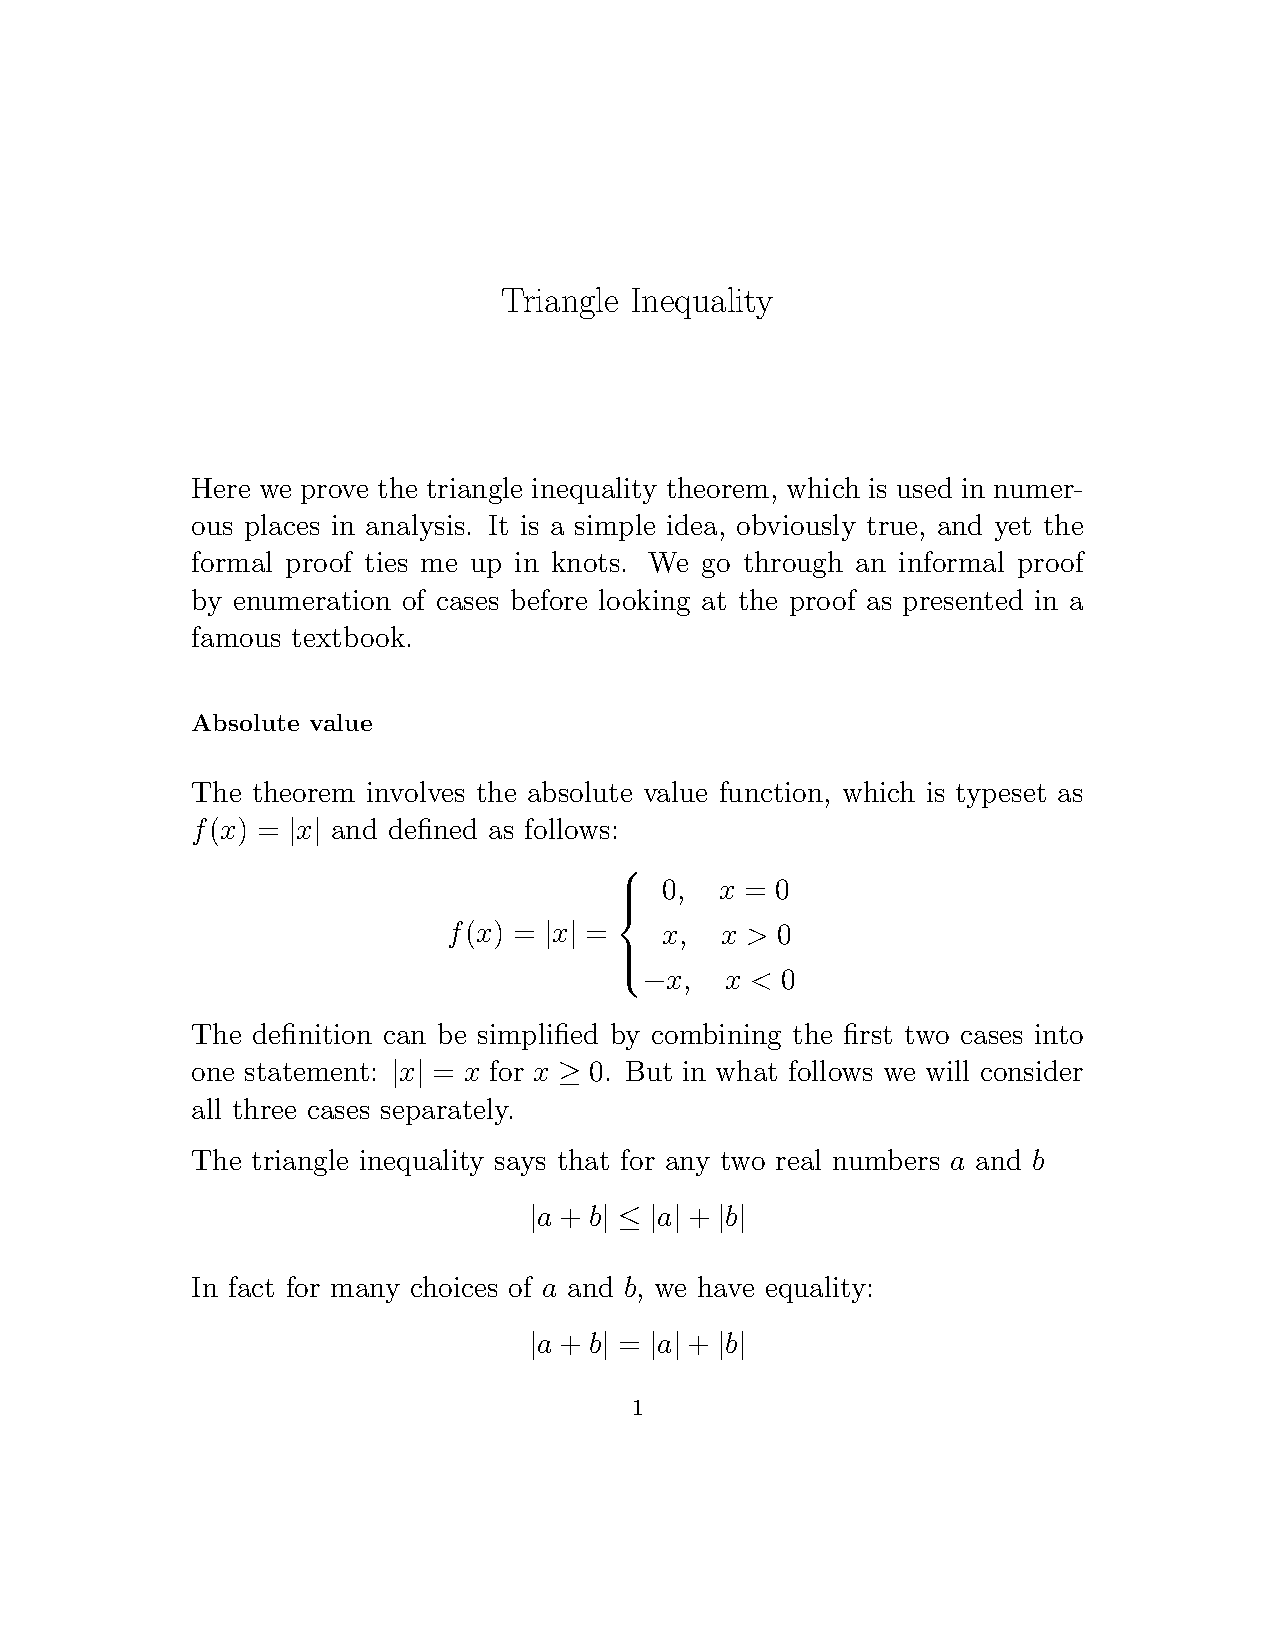
\includegraphics [scale=0.5] {triangle.png} \end{center}
\[ a^2 - e^2 = h^2 = b^2 - d^2 \]
So
\[ a^2 = e^2 + b^2 - d^2 \]
Since $d = c - e$ and thus $d^2 = c^2 - 2ce + e^2$:
\[ a^2 = e^2 + b^2 - (c^2 - 2ce + e^2) \]
\[ = b^2 - c^2 + 2ce  \]
but $e = a \cos B$ so
\[ a^2 = b^2 - c^2 + 2ac \cos B  \]
rearrange to give a more familiar form (this is the law of cosines)
\[ b^2 = a^2 + c^2 - 2ac \cos B  \]
Any side of a triangle can be expressed in terms of the other two and the cosine of the angle between them.  Thus, for example
\[ c^2 = a^2 + b^2 - 2ab \cos C  \]
\[ a^2 = b^2 + c^2 - 2bc \cos A  \]

Now, to compare with the dot product, label side $b$ as the vector $\mathbf{b}$ extending from vertex $A$ to $C$, similarly, label side $c$ as the vector $\mathbf{c}$ extending from vertex $A$ to $B$.  The angle between the two vectors is the angle $A$.
\begin{center} 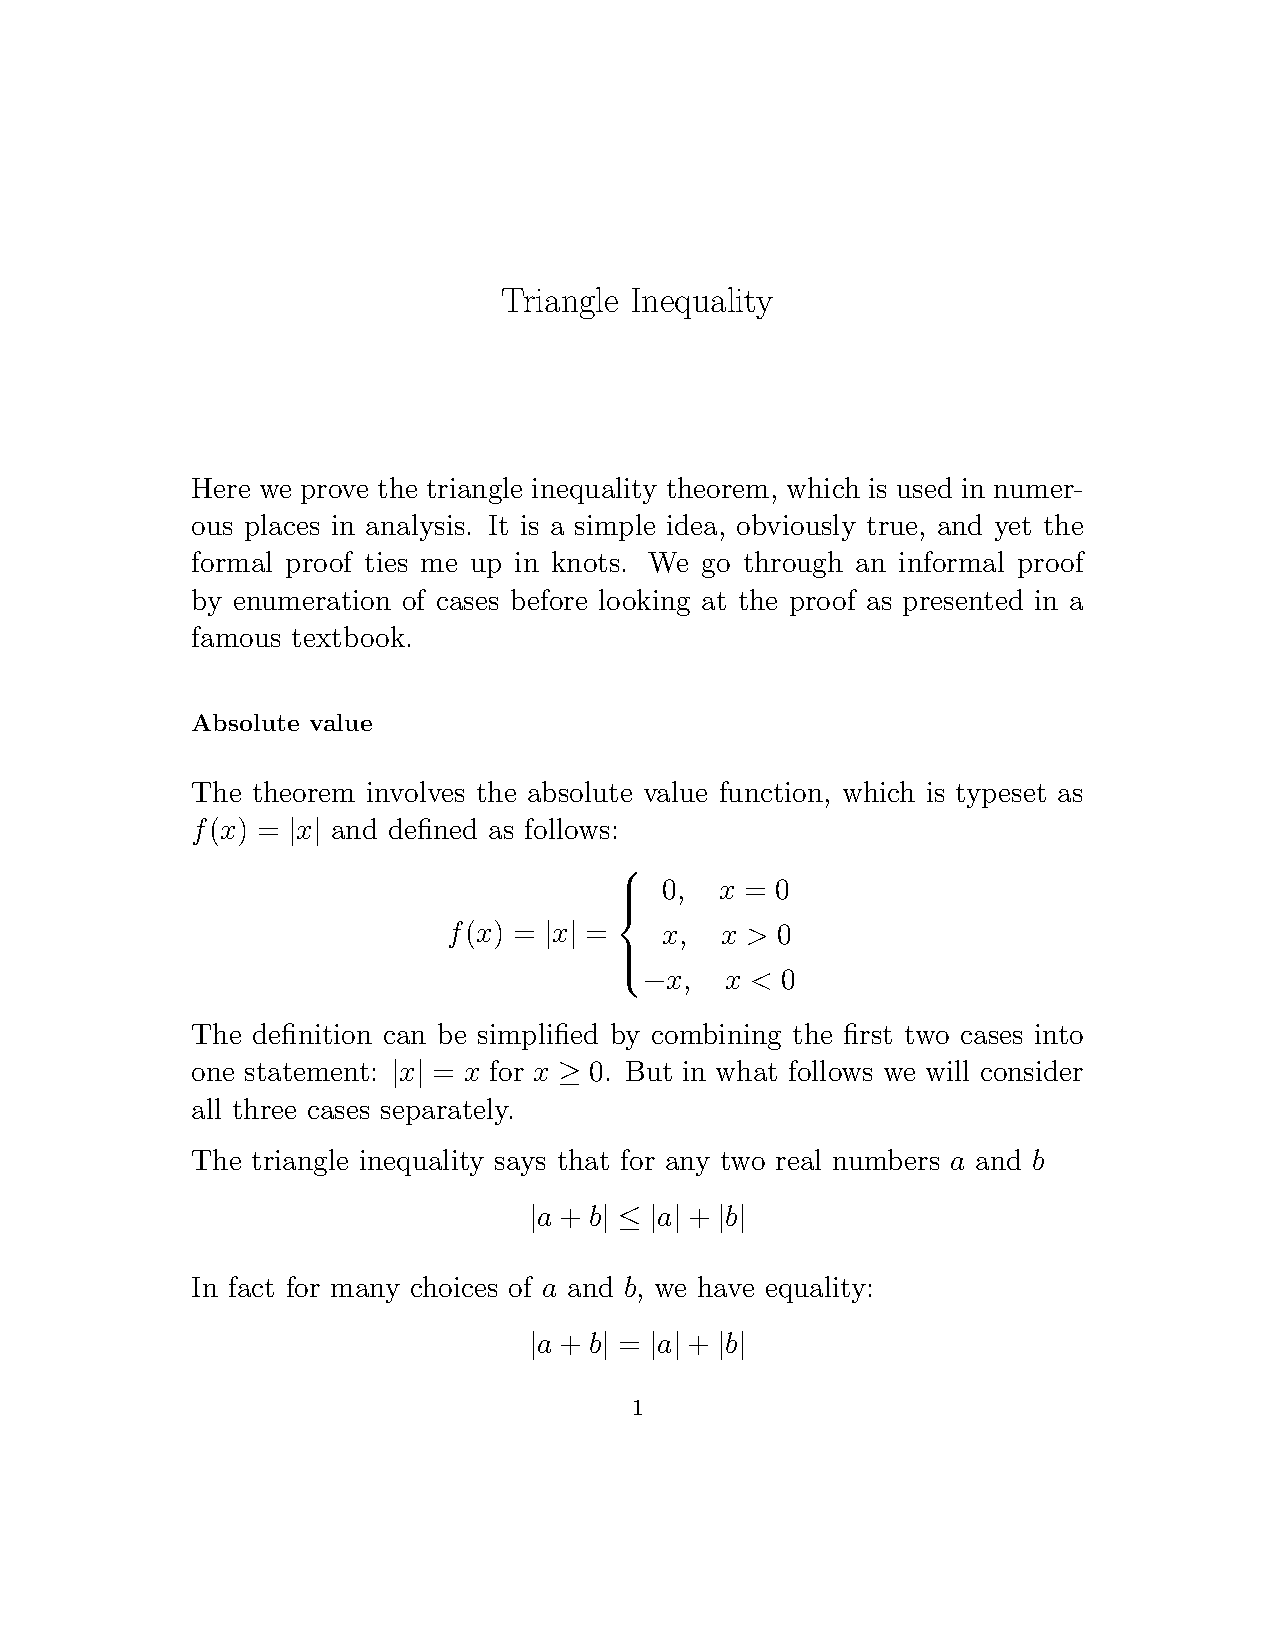
\includegraphics [scale=0.5] {triangle.png} \end{center}
If we view side $a$ as the vector $\mathbf{a}$, extending from vertex $C$ to $B$, then
\[ \mathbf{b} + \mathbf{a} = \mathbf{c} \]
\[ \mathbf{a} = \mathbf{c} - \mathbf{b} \]
The length of side $a$ squared is
\[ a^2 = \mathbf{a} \cdot \mathbf{a} \]
\[ = (\mathbf{c} - \mathbf{b}) \cdot (\mathbf{c} - \mathbf{b}) \]
\[ = \mathbf{c} \cdot \mathbf{c} - 2 \ \mathbf{c} \cdot \mathbf{b} + \mathbf{b} \cdot \mathbf{b} \]
\[ = c^2 + b^2 - 2 \ \mathbf{c} \cdot \mathbf{b} \]
Compare with the law of cosines and we see that
\[ \mathbf{c} \cdot \mathbf{b} = |\mathbf{c}| |\mathbf{b}| \cos A \]

One very useful property of the dot product is that it is easy to test whether two vectors are perpendicular (orthogonal) to each other, because in that case the dot product is zero.  It's also easy to find a vector that is orthogonal to a second vector, using the dot product as a guide.

We only proved it for $\mathbb{R}2$ but the last form of the dot product is true for all dimensions.

Finally (and also in $\mathbb{R}2$), let's examine the consequences of rotation of the coordinate system.  Recall that rotation of a vector by an angle $\theta$ in the counterclockwise direction can be achieved by this matrix multiplication
\[
\begin{bmatrix}  
\cos\  \theta & -\sin\  \theta  \\  
\sin\  \theta & \ \ \cos\  \theta  
\end{bmatrix}
\begin{bmatrix}  
x  \\  
y  
\end{bmatrix}
=
\begin{bmatrix}  
x\cos\  \theta - y \sin \theta \\  
x \sin\  \theta + y \cos \theta
\end{bmatrix}
\]
For example, the unit vector $\langle1,0\rangle$ becomes $\langle \cos \theta,\sin \theta \rangle$, and $\langle 0,1\rangle$ becomes $\langle -\sin \theta,\cos \theta \rangle$.  Counterclockwise rotation of vectors can also be viewed as a clockwise rotation of the coordinate system.  In other words, we can write
\[ x' = x\cos \theta - y \sin \theta \]
\[ y' = x \sin \theta + y \cos \theta \]
for clockwise rotation of coordinates (and to go the other way change the angle to be negative, which just changes the sign of the $\sin$ terms).

So if we have two vectors $\mathbf{a}$ and $\mathbf{b}$ in the standard coordinate system, the same vectors in a rotated coordinate system will be
\[ \mathbf{a}' = \ \langle a_x\cos \theta - a_y \sin \theta, a_x \sin \theta + a_y \cos \theta \rangle \]
\[ \mathbf{b}' = \ \langle b_x\cos \theta - b_y \sin \theta, b_x \sin \theta + b_y \cos \theta \rangle \]
Now, compute
\[ \mathbf{a}' \cdot \mathbf{b}' = a_x b_x \cos^2 \theta - a_x b_y \cos \theta \sin \theta - a_y b_x \sin \theta \cos \theta + a_y b_y \sin^2 \theta  \]
\[ \ \ \ \ \ \ \ \ \ + a_x b_x \sin^2 \theta + a_x b_y \sin \theta \cos \theta + a_y b_x \cos \theta \sin \theta + a_y b_y \cos^2 \theta \]
All the terms containing $a_x b_y$ and $a_y b_x$ cancel, which leaves
\[ = a_x b_x \cos^2 \theta + a_y b_y \sin^2 \theta + a_x b_x \sin^2 \theta + a_y b_y \cos^2 \theta \]
and the terms $a_x b_x$ and $a_y b_y$ can be factored out of $\sin^2 \theta + \cos^2 \theta$, giving
\[ = a_x b_x + a_y b_y \]
As expected, we obtain the same dot product for the vectors in the rotated coordinate system.  Viewed in another way, any two vectors which are rotated but maintain the same angle between them, will have the same dot product.

\subsection*{cross product}

Now we'll look at the cross-product.  

Suppose we have two ordinary vectors $\mathbf{u}$ and $\mathbf{v}$.  These must be in $\mathbb{R}3$ because the cross-product is only defined for vectors in $\mathbb{R}3$.

We write the cross-product as
\[ \mathbf{u} \times \mathbf{v} = \mathbf{w}  \]
The simplest definition is that the magnitude of $\mathbf{w}$ is 
\[ |\mathbf{w}| = |\mathbf{u}| |\mathbf{v}| \sin \theta \]
The symmetry with the dot product is obvious.  

The direction is defined by saying that $\mathbf{w}$ is orthogonal to the plane which contains both $\mathbf{u}$ and $\mathbf{v}$, and its sign is given by the right-hand rule.  Curl the fingers of your right hand around in the direction from $\mathbf{u}$ to $\mathbf{v}$.  Your thumb points in the direction of $\mathbf{w}$.  

The term $\sin \theta$ means that the cross-product of any vector with itself is zero.
\[ \mathbf{a} \times \mathbf{a} = \mathbf{0}  \]

To make the notation simpler, we define
\[ \mathbf{u} = \langle p,q,r \rangle \]
\[ \mathbf{v} = \langle x,y,z \rangle \]
and in order to compute the cross product, we form what looks like a really weird matrix
\[
\begin{bmatrix} 
  i  &  j  &  k \\ 
  p  &  q & r \\
  x  &  y & z
\end{bmatrix}
\]
and calculate its "determinant"
\[ \mathbf{u} \times \mathbf{v}  = (qz - ry) \ \hat{\mathbf{i}} + (rx - pz) \  \hat{\mathbf{j}}  + (py - qx) \ \hat{\mathbf{k}}  \]
We can show that the resulting vector is orthogonal to the two starting vectors, $\mathbf{u}$ and $\mathbf{v}$.  Test that by forming the usual, dot product with $\mathbf{u}$.
\[ \mathbf{u} \cdot (\mathbf{u} \times \mathbf{v})  =  p(qz - ry) + q(rx - pz)   + r(py - qx)  \] 
The first and fourth terms cancel, the second and fifth terms cancel, and the third and sixth terms also cancel.  

So $\mathbf{u} \cdot (\mathbf{u} \times \mathbf{v}) = 0$, and $\mathbf{v} \cdot (\mathbf{u} \times \mathbf{v}) = 0$ as well.  In fact, we use the cross-product to find the normal vector a plane in vector calculus.

As an aside, we could have skipped this calculation.  The following rule holds for vectors:
\[ \mathbf{a} \cdot ( \mathbf{b} \times \mathbf{c} ) = ( \mathbf{a} \times \mathbf{b} ) \cdot \mathbf{c} \]
(we will explore triple products below).
So
\[ \mathbf{u} \cdot (\mathbf{u} \times \mathbf{v}) = (\mathbf{u} \times \mathbf{u}) \cdot \mathbf{v} = 0 \]
\[ \mathbf{v} \cdot (\mathbf{u} \times \mathbf{v}) = - \mathbf{v} \cdot (\mathbf{v} \times \mathbf{u}) = - (\mathbf{v} \times \mathbf{v}) \cdot \mathbf{u}) = 0 \]

\subsection*{About the angle}

How to show that

\[ \mathbf{a} \times \mathbf{b} = |\mathbf{a}| |\mathbf{b}| \sin \theta \ \hat{\mathbf{n}}  \]

where $\hat{\mathbf{n}}$ is perpendicular to $\mathbf{a}$ and $\mathbf{b}$.

\[ |\mathbf{a} \times \mathbf{b} | = |\mathbf{a}| |\mathbf{b}| \sin \theta \]

According to wikipedia, this is the \emph{definition} of the cross-product, and from this one can derive the expression that we got by setting up our matrix and computing its "determinant."  So that is what we are going to do.


In the wikipedia article on the cross-product, this formula is given:

\[ | \mathbf{a} \times \mathbf{b} |^2 + (\mathbf{a} \cdot \mathbf{b})^2 = |\mathbf{a}|^2 |\mathbf{b}|^2 \]

Starting from 
\[ \mathbf{a} \cdot \mathbf{b}  = |\mathbf{a}| |\mathbf{b}| \cos \theta \]
\[ |\mathbf{a} \times \mathbf{b} | = |\mathbf{a}| |\mathbf{b}| \sin \theta \]

Then we have
\[ (\mathbf{a} \cdot \mathbf{b} )^2 = |\mathbf{a}|^2 |\mathbf{b}|^2 \cos^2 \theta \]
\[ |\mathbf{a} \times \mathbf{b} |^2 = |\mathbf{a}|^2 |\mathbf{b}|^2 \sin^2 \theta \]
\[ | \mathbf{a} \times \mathbf{b} |^2 + (\mathbf{a} \cdot \mathbf{b})^2 = |\mathbf{a}|^2 |\mathbf{b}|^2 \]

That looks very promising.  Now we know what we have to do.

I am going to go back to the notation we had before, rather than use subscripts like $a_x$, etc.

\[ \mathbf{u} = \langle p,q,r \rangle \]
\[ \mathbf{v} = \langle x,y,z \rangle \]

So

\[ \mathbf{u} \times \mathbf{v}  = (qz-ry) \hat{\mathbf{i}}  + (rx-pz) \hat{\mathbf{j}} + (py-qx) \hat{\mathbf{k}}\]

\[ |\mathbf{u} \times \mathbf{v}|^2 = (qz-ry)^2 + (rx-pz)^2 + (py-qx)^2 \]
\[ = (qz)^2 - 2qryz + (ry)^2 + (rx)^2 - 2prxz + (pz)^2 + (py)^2 - 2pqxy + (qx)^2 \]


\[ \mathbf{u} \cdot \mathbf{v} = px + qy + rz \]
\[ (\mathbf{u} \cdot \mathbf{v})^2 = (px)^2 + (qy)^2 + (rz)^2 + 2pqxy + 2prxz + 2qryz \]

When we add these together, all the terms with cofactor $2$ cancel so that leaves

\[ | \mathbf{u} \times \mathbf{v} |^2 + (\mathbf{u} \cdot \mathbf{v})^2 \]
\[ =  (qz)^2 + (ry)^2 + (rx)^2 + (pz)^2 + (py)^2 + (qx)^2 + (px)^2 + (qy)^2 + (rz)^2 \]


rearranging terms
\[ = (px)^2 + (py)^2 + (pz)^2 + (qx)^2 + (qy)^2 + (qz)^2 + (rx)^2 +(ry)^2   + (rz)^2 \]

\[ = (p^2 + q^2 + r^2)(x^2 + y^2 + z^2) \]

\[ = |\mathbf{u}|^2 |\mathbf{v}|^2 \]

That was tedious, but it we made it.

All these properties of the cross-product are connected.
\[ \mathbf{a}  \cdot (\mathbf{a} \times \mathbf{b}) = \mathbf{b}  \cdot (\mathbf{a} \times \mathbf{b}) = 0 \]
\[ \mathbf{a} \times \mathbf{b} =  \ \langle qu-rt, rs-pu, pt-qs \rangle \]
\[ |\mathbf{a} \times \mathbf{b}|  = |\mathbf{a}| |\mathbf{b}| \sin \theta \]
\[ | \mathbf{a} \times \mathbf{b} |^2 + (\mathbf{a} \cdot \mathbf{b})^2 = |\mathbf{a}|^2 |\mathbf{b}|^2 \]

\subsection*{Triple products}
Suppose we have
\[\mathbf{a} = \ \langle p,q,r \rangle \]
\[\mathbf{b} = \ \langle s,t,u \rangle \]
\[\mathbf{c} = \ \langle x,y,z \rangle \]
And
\[ \mathbf{a} \times \mathbf{b} =  \ \langle qu-rt, rs-pu, pt-qs \rangle \]
\[ \mathbf{b} \times \mathbf{c} =  \ \langle tz-uy, ux-sz, sy-tx \rangle \]
\[ \mathbf{a} \times \mathbf{c} =  \ \langle qz-ry, rx-pz, py-qx \rangle \]
Algebraically
\[ \mathbf{a} \cdot (\mathbf{b} \times \mathbf{c}) = p(tz-uy) + q(ux-sz) + r(sy-tx)  \]
\[ \mathbf{b} \cdot (\mathbf{c} \times \mathbf{a}) = s(ry-qz) + t(pz-rx) + u(qx-py) \]
\[ \mathbf{c} \cdot (\mathbf{a} \times \mathbf{b}) = x(qu-rt) + y(rs-pu) + z(pt-qs) \]
So
\[ \mathbf{a} \cdot (\mathbf{b} \times \mathbf{c}) = \mathbf{b} \cdot (\mathbf{c} \times \mathbf{a}) = \mathbf{c} \cdot (\mathbf{a} \times \mathbf{b}) \]

The way to remember this is that these are all the same cyclic permutation.

A much simpler proof is to remember that the cross-product $\mathbf{a} \times \mathbf{b}$ is the area of the parallelogram formed by $\mathbf{a}$ and $\mathbf{b}$ and the \emph{scalar} triple product is the signed volume of the parallelipiped formed by the three vectors.   Signed meaning that $\mathbf{c} \cdot (\mathbf{a} \times \mathbf{b}) = -\mathbf{c} \cdot (\mathbf{b} \times \mathbf{a})$ so the area may come out negative, if we order $\mathbf{a}$ and $\mathbf{b}$ differently.

\begin{center} 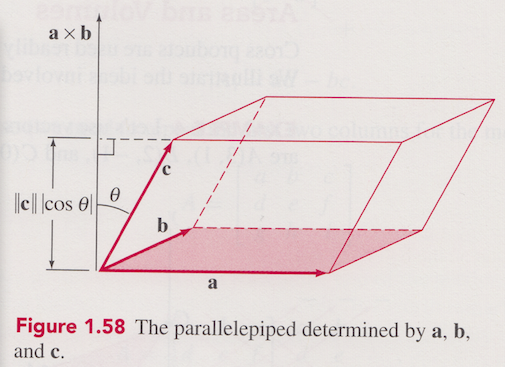
\includegraphics [scale=0.5] {ppd_volume.png} \end{center}
\begin{flushright}Colley \emph{Vector Calculus}\end{flushright}

Recall that the direction of $\mathbf{a} \times \mathbf{b}$ is perpendicular to both vectors.   If we are careful to write the cross-product in the correct order using the right-hand rule, the result of the dot product will always be positive, with the projection of $\mathbf{c}$ onto the cross-product equal to the height of the solid.  In particular, for this arrangement, we must write $\mathbf{a} \times \mathbf{b}$, $\mathbf{b} \times \mathbf{c}$, or $\mathbf{c} \times \mathbf{a}$.

It doesn't matter which two vectors we choose as the base of our solid, the volume must come out the same.
\[ \mathbf{a} \cdot (\mathbf{b} \times \mathbf{c}) = \mathbf{b} \cdot (\mathbf{c} \times \mathbf{a}) = \mathbf{c} \cdot (\mathbf{a} \times \mathbf{b}) \]

The other triple product is
\[ \mathbf{a} \times (\mathbf{b} \times \mathbf{c}) = \]
The components are, in order,
\[ q(sy-tx) - r(ux-sz) \]
\[ r(tz-uy) - p(sy-tx) \]
\[ p(ux-sz) - q(tz-uy) \]
"BACK CAB"
\[ = \mathbf{b} (\mathbf{a} \times \mathbf{c}) - \mathbf{c} (\mathbf{a} \times \mathbf{b}) \]

needs more work

\subsection*{Kepler and time-derivatives}
Continuing with the Kepler problem, the vectors that we are thinking about are special.  The vectors (and their components) are functions of time.  For example,

\[ \mathbf{r}(t) = \langle x(t), y(t), z(t) \rangle \]

At any particular time $t$, we get three numbers, and $\mathbf{r}$ reduces to a vector of the familiar type.  We should keep this in mind, it's why it makes sense to take the derivative with respect to time of $\mathbf{r}$, but we will drop the $(t)$ to make the notation simpler.  So

\[ \mathbf{r} = \langle x, y, z \rangle \]

A second simplification to the notation is to use the dot notation to denote the time derivative, which we do term by term in the vector.  For example:

\[ \mathbf{v} = \frac{d}{dt} \mathbf{r} =  \dot{\mathbf{r}} = \langle  \dot{x},\dot{y},\dot{z} \rangle \]

So now we want to compute 

\[ \frac{d}{dt} (\mathbf{r} \times \mathbf{v}) =  \frac{d}{dt} (\mathbf{r} \times \dot{\mathbf{r}} ) \]

Set up the matrix as before

\[
\begin{bmatrix} 
  i  &  j  &  k \\ 
  x  &  y & z \\
  \dot{x}  &  \dot{y} & \dot{z}
\end{bmatrix}
\]

and compute the "determinant."

\[ (y \dot{z} - \dot{y} z) \hat{\mathbf{i}}  + (\dot{x}z - x\dot{z} )  \hat{\mathbf{j}}  + (x \dot{y} - \dot{x} y)  \hat{\mathbf{k}}  \]

The critical step is to now compute the time-derivative, but we just follow our rules.  First, we go through the vector one component at a time.  For each component we have two terms, and each term is the product of two ordinary functions.  So we use the standard product rule, and obtain

\[ \frac{d}{dt} (\mathbf{r} \times \dot{\mathbf{r}} ) = \frac{d}{dt} \ [ \ (y \dot{z} - \dot{y} z) \hat{\mathbf{i}}  + (\dot{x}z - x\dot{z} )  \hat{\mathbf{j}}  + (x \dot{y} - \dot{x} y)  \hat{\mathbf{k}} \ ]  \]

\[ = (\dot{y} \dot{z} + y \ddot{z} - \ddot{y} z - \dot{y}\dot{z}) \hat{\mathbf{i}} + 
(\ddot{x}z + \dot{x} \dot{z} - \dot{x}\dot{z} - x\ddot{z}) \hat{\mathbf{j}} +
(\dot{x} \dot{y} + x \ddot{y} - \ddot{x} y - \dot{x}\dot{y}) \hat{\mathbf{k}} 
\]
  
Notice that each component has two terms that cancel.  If you set up the matrix you will see that these are the terms that arise from $\dot{\mathbf{r}} \times \dot{\mathbf{r}}$.  The terms that remain are then

\[ = (y \ddot{z} - \ddot{y} z) \hat{\mathbf{i}} + 
( \ddot{x}z - x\ddot{z}) \hat{\mathbf{j}} +
( x \ddot{y} - \ddot{x} y) \hat{\mathbf{k}} 
\]

which I hope you will recognize as resulting from $\mathbf{r} \times \ddot{\mathbf{r}}$.  In summary, by going through term by term, we have shown that

\[ \frac{d}{dt} (\mathbf{r} \times \dot{\mathbf{r}} ) = \mathbf{r}\times \ddot{\mathbf{r}} + \dot{\mathbf{r}} \times \dot{\mathbf{r}}  =  \mathbf{r}\times \ddot{\mathbf{r}} \]

\subsection*{Product rule for the dot product}

Going back to differentiation, it's worth mentioning that this is also true for the dot product:

\[ \frac{d}{dt} (\mathbf{u} \cdot \mathbf{v}) = \dot{\mathbf{u}}  \cdot \mathbf{v} + \mathbf{u} \cdot \dot{\mathbf{v}} \]

As before, the components are

\[ \mathbf{u} = \langle p,q,r \rangle \]
\[ \mathbf{v} = \langle x,y,z \rangle \]

\[ \mathbf{u} \cdot \mathbf{v} = px + qy + rz \]

By the standard product rule, the time-derivative is

\[ \frac{d}{dt} (\mathbf{u} \cdot \mathbf{v}) = \dot{p}x + x \dot{p} + \dot{q}y + q \dot{y} + \dot{r}z + r \dot{z} \]
\[ = (\dot{p}x + \dot{q}y + \dot{r}z) + (x \dot{p} + q \dot{y} + r \dot{z}) \]
\[ = (\dot{\mathbf{u}}  \cdot \mathbf{v}) + (\mathbf{u} \cdot \dot{\mathbf{v}}) \] 


\end{document}  